
\documentclass[10pt]{beamer}

\usetheme[progressbar=frametitle]{metropolis}
\usepackage{appendixnumberbeamer}
\usepackage[numbers,sort&compress]{natbib}
\bibliographystyle{plainnat}

\usepackage{booktabs}
\usepackage[scale=2]{ccicons}
\DeclareGraphicsExtensions{.pdf,.png,.jpg}
\usepackage{xspace}
\newcommand{\themename}{\textbf{\textsc{metropolis}}\xspace}
\title{Sistema para administrar una clínica}
 \subtitle{Algoritmos Computacionales}
% \date{\today}
\date{3 de Junio 2019}
\author{De la Torre Morales Ma.Fernanda. \\
Martinez Gutierrez Berenice Anahi. \\
Santos Sanchez Betsabe. \\
}
%\institute{UFPR - Disciplina - Semestre}
% \titlegraphic{\hfill\includegraphics[height=1.5cm]{logo.pdf}}

\begin{document}

\maketitle

\begin{frame}{Tabla de contenidos}
  \setbeamertemplate{section in toc}[sections numbered]
  \tableofcontents[hideallsubsections]
\end{frame}

\section{Introducción}
\begin{frame}[fragile]{Introducción}

  Python es un lenguaje de programación multiparadigma. Puede ser usado para realizar cualquier tipo de programa, desde calculos matemáticos, aplicaciones o incluso, páginas web.
  
  Python se puede utilizar en aplicaciones de base de datos


  Basado en lo visto en clase, se pudo desarollar un sistema que permite administrar una clínica donde se le permite a los usuarios realizar diferentes actividades según su rol en la clínica, como pueden ser paciente, secretaria o doctor.
  
  \begin{figure}[t]
    \raggedleft
    
\includegraphics[width=3cm]{logopy.png}
  \end{figure}

\end{frame}

\begin{frame}[fragile]{¿Por qué bases de datos?}

  Una base de datos es un “almacén” que nos permite guardar grandes cantidades de información
  de forma organizada para que luego podamos encontrar y utilizar fácilmente.
  
  
  
  \centering
  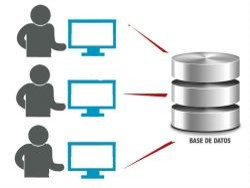
\includegraphics[width=5cm]{Python2.jpg}
  
  
\end{frame}

\section{Objetivos}
\begin{frame}{Objetivos}
    Se tuvo como objetivos: \\
    \begin{itemize}
        \item Implementat un sistema de 
        administración de una clínica usando Python y bases de datos. \\
        \item Generar usuarios (doctores, secretarias,  pacientes y adminis). \\
        \item Establecer permisos para cada usuario. \\ 
        \item Permitir al usuario realizar actividades con relación a su rol. \\
    \end{itemize}
    
\end{frame}

\section{Metodología}
\begin{frame}[fragile]{Metodología}
1. Identificar las prioridades/características del sistema para clínica \\
2. Realizar una base de datos con MySQL. \\
3. Backend \\
4. Ocupar Pandas para analizar datos. \\
5. Manipulación de datos. \\
6. Dar diseño a las ventanas para el sistema de administración de una clínica. \\
\end{frame}

\begin{frame}{1. Identificar las prioridades/características del sistema para clínica}
 \\
\begin{itemize}
    \item[$\rightarrow$] Actualización de la base de datos. \\
    \item[$\rightarrow$] Agilizar la consulta de los datos. \\
     \item[$\rightarrow$] Generar un historial de pacientes \\
    \item[$\rightarrow$] Que el sistema sea fácil y eficaz. \\
\end{itemize}
\end{frame}

\begin{frame}{2. Realizar una base de datos con MySQL}
MySQL es un sistema de gestión de base de datos de código abierto, basado en lenguaje de consulta estructurado (SQL).
SQL, Structure Query Language (Lenguaje de Consulta Estructurado) es un lenguaje de programación para trabajar con base de datos relacionales como MySQL.

\centering

\includegraphics[width=4cm]{mysql.png}

\end{frame}
\begin{frame}{Base de datos con MySQL}

\centering
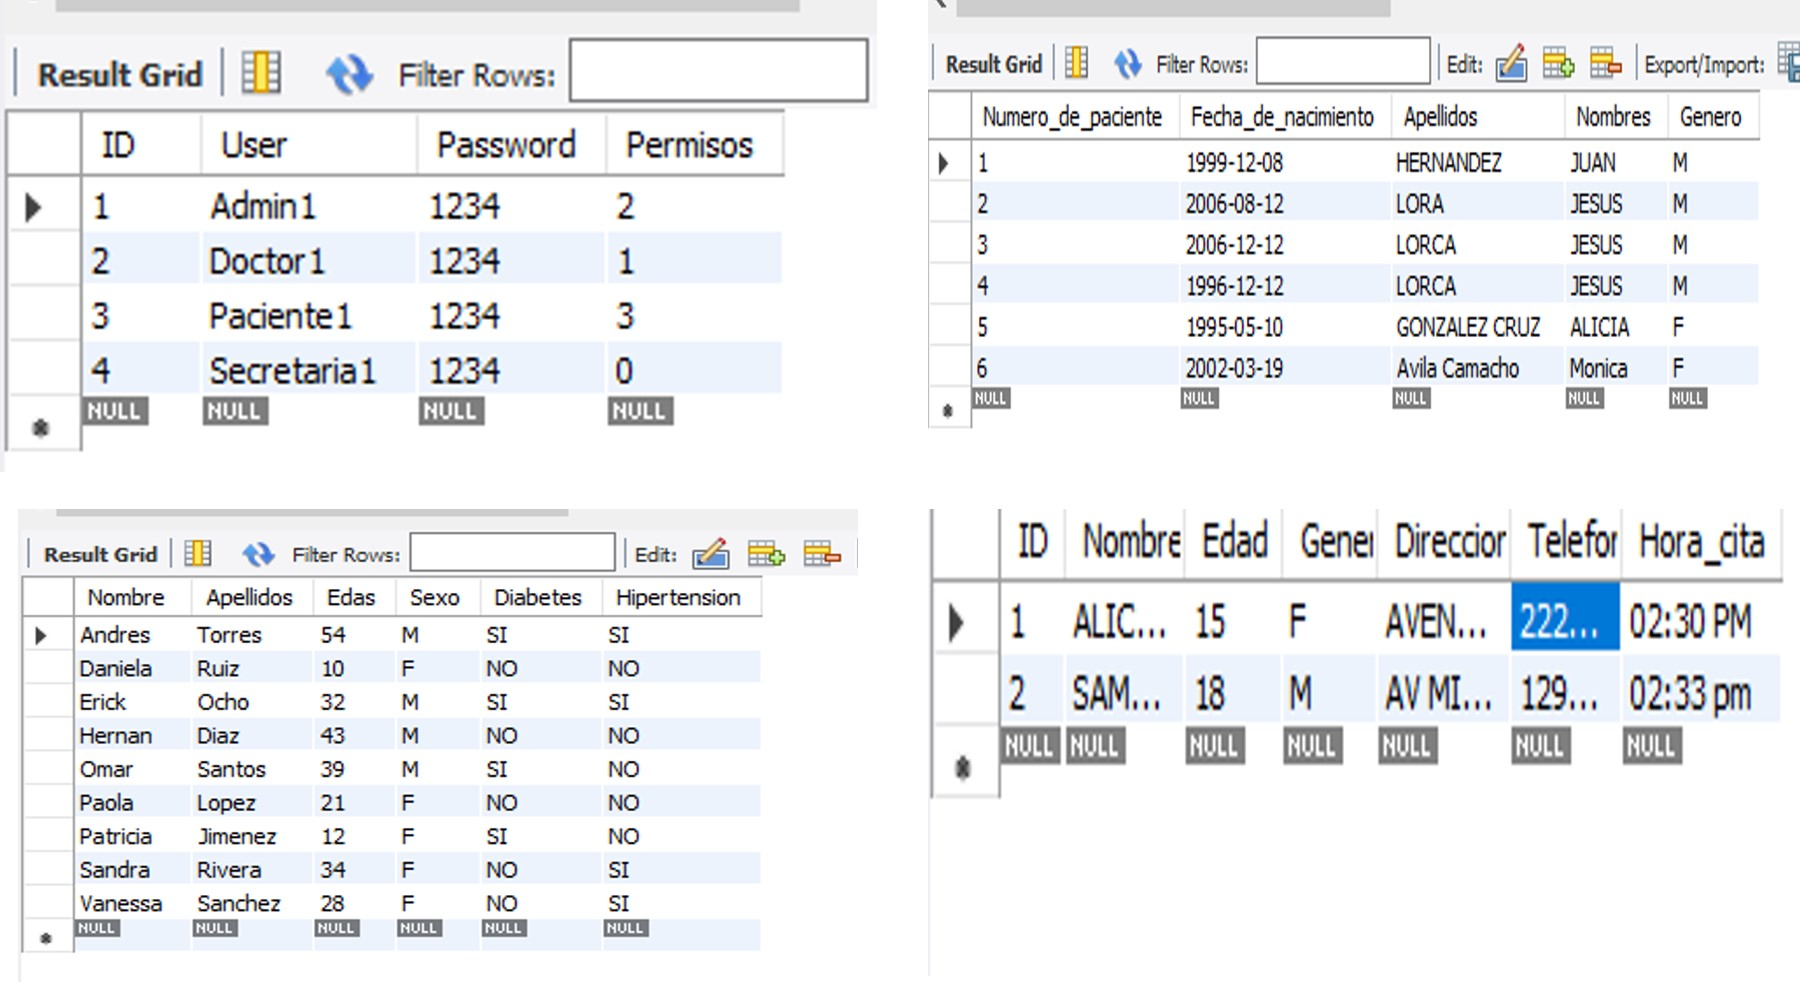
\includegraphics[width=11cm,]{junto.jpg}




\end{frame}



\begin{frame}{3. Backend}

El backend es la parte del desarrollo  que se encarga de que toda la lógica de una página web o aplicación  funcione. Conjunto de acciones que que no vemos en una interfaz como, por ejemplo, la comunicación con el servidor o en esta caso la Base de Datos.


Existen comandos especiales para el manejo de sistemas de base de datos. Los cursores son una herramienta de SQL que nos permite recorrer el resultado de una consulta SQL y realizar operaciones en cada paso de ésta.  Nos permite realizar consultas a nuestras bases de datos, para mostrar, insertar, actualizar y borrar datos. (Select * From , Insert. Insert Into, Delete) 


\end{frame}

\begin{frame}{4. Ocupar pandas para analizar datos}
Pandas es una librería que permite usar o crear tablas de datos y a partir de ellas manipular sus datos, pandas además permite adicionar filas o columnas, seleccionar solo los datos deseados y con estos poder hacer graficas para su comparación. \\
\centering

\includegraphics[width=5cm]{pandas.jpg}
\end{frame}


\begin{frame}{5. Manipulacion de datos}

Agregar columnas

Seleccionar ciertas columnas o filas

Gráficas para medir la cantidad de población con cierta enfermedad o requisito

\end{frame}

\begin{frame}{6. Programación orientada a objetos}
Paradigma de programación que proporciona un medio de estructuración de programas para que las propiedades y comportamientos se empaqueten en objetos individuales.
Trata de modelar cosas del mundo real. 

* Instancias

*Clases

*Atributos

*Herencia


\centering

\includegraphics[width=4cm]{Post-Persona.jpg}
\end{frame}

\begin{frame}{7. Clases }
Las clases se utilizan para crear nuevas estructuras de datos definidas por el usuario que contengan información arbitraria sobre algo. 


\end{frame}

\begin{frame}{8. Despliegue de ventanas}
Tomando en cuenta las tablas creadas:

\centering
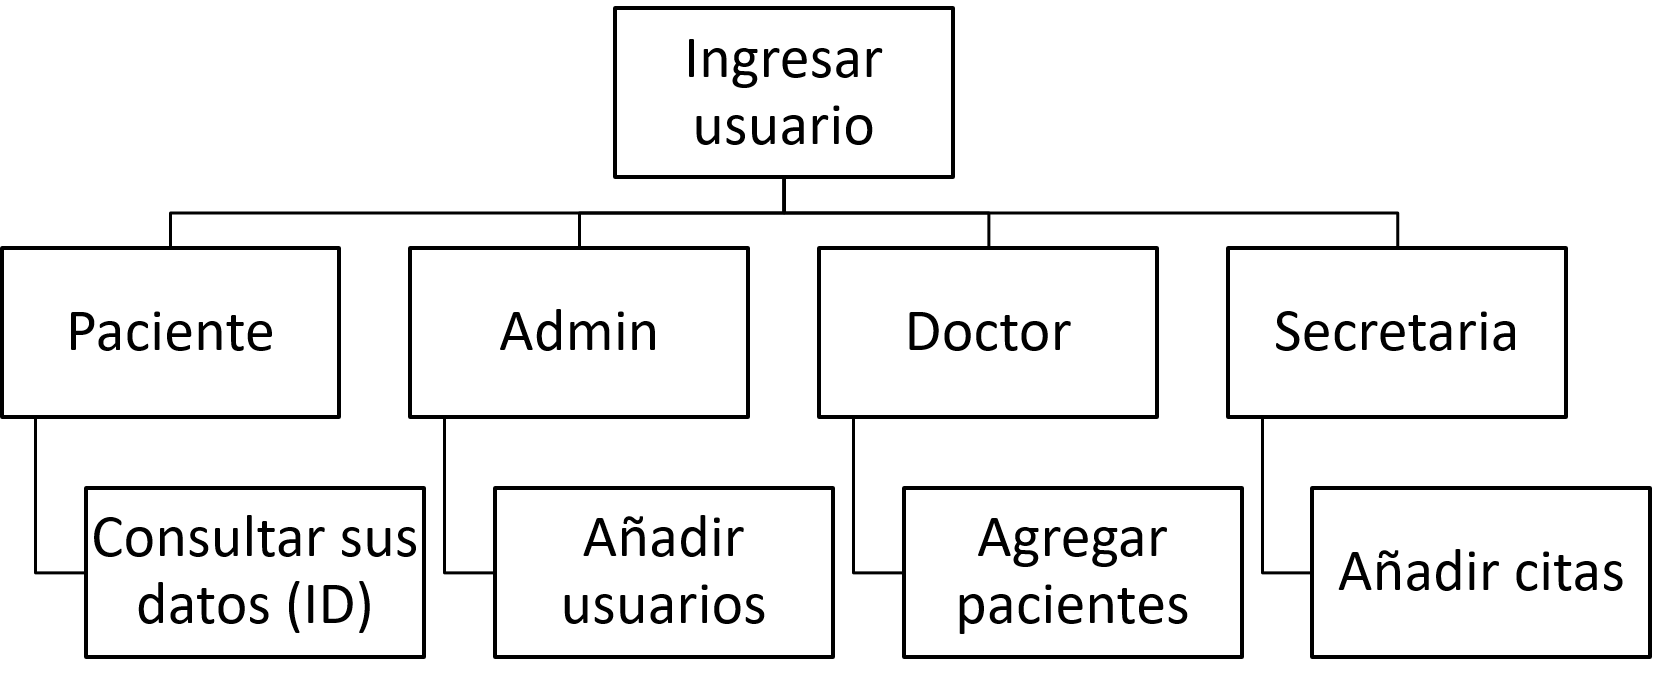
\includegraphics[width=10cm]{PYTHON1.png}
\end{frame}

\begin{frame}{9. Representación sencilla}
La interfaz gráfica de usuario, es un programa informático que actúa de interfaz de usuario, utilizando un conjunto de imágenes y objetos gráficos para representar la información y acciones disponibles en la interfaz. 

\centering
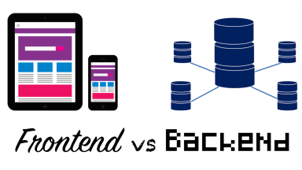
\includegraphics[width=5.5cm]{frontend.png}
\end{frame}

\begin{frame}{10. Tkinter}
El módulo Tkinter es una interfaz estándar de Python para TK GUI toolkit de Scriptics. 
La interfaz Tk proviene de la extensión binaria de otro módulo. 

\end{frame}

\section{Resultados}
\begin{frame}{Resultados}
Se diseñaron diferentes ventanas con base de datos que le permiten a usuarios de diversos roles (doctor, secretaria o paciente), manipular diversos datos segun los permisos que tenga el usuario.
\end{frame}


\begin{frame}{Programa (interfaz)}
Se corre desde la consolo con comando python

\centering
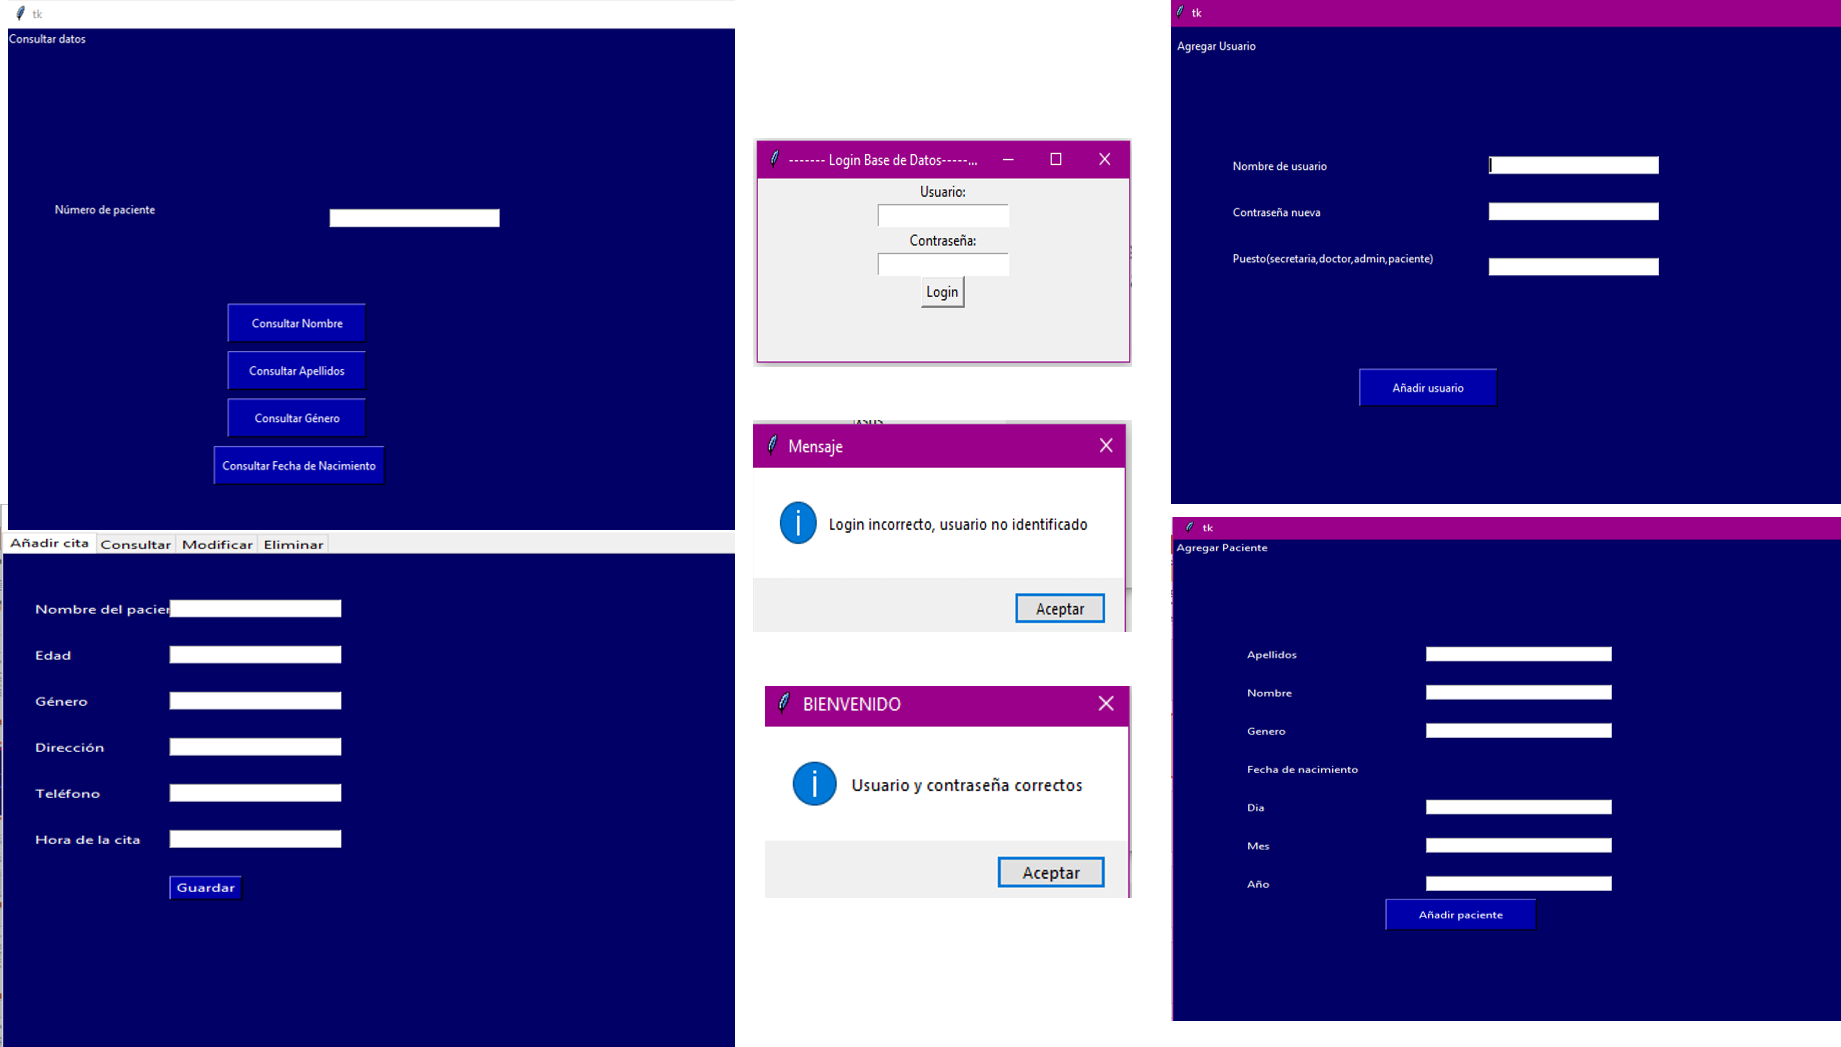
\includegraphics[width=12cm]{ventas.png}
 
\end{frame}

\section{Conclusiones}
\begin{frame}{Conclusiones}
- Se otorgó acceso  para cada usuario segun su rol. \\
- Se logro desarrollar un sistema que permita a una clinica manipular diferentes datos segun los permisos otorgados al usuario. \\
- Se diseño un sistema de fácil uso para el usuario. \\
\end{frame}

\section{Trabajo a futuro}
\begin{frame}{Trabajo a futuro}
* Se pretende probar el sistema en un servidor. \\
* Continuar el sistema de administración para una clinica. \\
* Crear documentos con los resulados de los análisis clínicos. \\
* Anexar el documento para poder generar recetas médicas. \\
* Incrementar el uso de pandas para realizar gráficos. \\
\end{frame}

\section{Referencias}
\begin{frame}{Referencias}
KLINE, K., GOULD, L. and ZANEVSKY, A. (1999). \textit{Transact-SQL programming} Beijing [etc.]: O'Reilly. \\
[2] CUEVAS ÁLVAREZ, A. (2016). \textit{ Python 3.} Paracuellos del Jarama, Madrid: Ra-Ma.\\
[3] GRUS, J. (2019). \textit{Data science from scratch}. [Place of publication not identified]: O'REILLY MEDIA.
\end{frame}
\end{document}
